\chapter{Renta variable (Equity)}\label{cap:equity}

\section{El mercado}
Se negocian acciones individuales, índices (vía futuros como ES/NQ/FESX, ETFs como SPY/QQQ, o CFD),
sectores y opciones. Rasgos propios:
\begin{itemize}
\item \textbf{Deriva positiva a largo plazo} (prima de riesgo de la renta variable de 4--6~\% anual): ir
  corto es nadar contra corriente y requiere pedir prestado el título (coste de préstamo, riesgo de
  \emph{recall} y de \emph{short squeeze}).
\item \textbf{Eventos corporativos}: resultados trimestrales (gaps de $\pm5$--$15~\%$), dividendos,
  ampliaciones, splits, OPAs. El calendario de resultados es imprescindible.
\item \textbf{Asimetría de volatilidad}: las caídas son más rápidas y volátiles que las subidas; la
  volatilidad implícita (VIX) sube cuando el mercado baja.
\item \textbf{Fuerte factor común}: la mayoría de las acciones tienen beta positiva con el índice.
\end{itemize}

\section{Beta, CAPM y alfa}
La beta mide la sensibilidad al mercado:
\begin{equation}
\beta_i = \frac{\operatorname{Cov}(r_i,r_m)}{\operatorname{Var}(r_m)},\qquad
r_i - r_f = \alpha + \beta_i(r_m-r_f)+\varepsilon .
\end{equation}
(\py{equity.beta}, \py{equity.capm}). Una cartera de 10 acciones de beta 1,4 es, en gran parte, una
apuesta apalancada al índice. Para aislar la idea específica (\emph{alfa}) se cubre la beta vendiendo
$\beta\cdot$nocional del futuro del índice.

\paragraph{Factores.} Más allá del mercado, las rentabilidades se explican por factores como tamaño
(SMB), valor (HML), momentum (12--1 meses), calidad/rentabilidad y baja volatilidad.
\py{equity.factor\_regression} estima la exposición de una estrategia a factores; si tu «alfa»
desaparece al añadir el momentum, no tenías alfa, tenías momentum.

\paragraph{Momentum 12--1.} Rentabilidad de los últimos 12 meses excluyendo el último
(\py{equity.momentum\_12\_1}); el último mes muestra reversión a corto plazo.

\section{Setups habituales}
\begin{description}
\item[Ruptura con volumen.] Salida de un rango tras compresión de volatilidad, con volumen relativo
  alto. Stop bajo el rango; funciona mejor en régimen alcista del índice.
\item[Pullback en tendencia.] Retroceso a la media de 20/50 en una acción líder (fuerza relativa alta).
\item[Gap tras resultados.] Los gaps con sorpresa de beneficios grande tienden a continuar (\emph{post-earnings
  announcement drift}); los gaps sin noticia en acciones grandes tienden a cerrarse más
  (\py{equity.gap\_stats} mide la tasa de cierre).
\item[Reversión a corto plazo.] RSI(2) extremo en acciones/índices en tendencia alcista.
\end{description}

\section{Trading de pares (valor relativo)}
Dos acciones con el mismo negocio (KO/PEP, bancos de un mismo país) pueden estar
\textbf{cointegradas}: aunque cada precio es un paseo aleatorio, una combinación es estacionaria.
\begin{enumerate}
\item Estimar $\beta$ en $\ln y_t = a + \beta\ln x_t + s_t$ \emph{con datos pasados} (\py{equity.hedge\_ratio}).
\item Contrastar estacionariedad del spread $s_t$ (Dickey--Fuller, \py{equity.adf\_tstat}; con $\beta$
  estimado el crítico al 5~\% es $\approx -3{,}34$).
\item Vida media de reversión del AR(1) $\Delta s_t = a + b\,s_{t-1}$: $HL = -\ln 2/\ln(1+b)$
  (\py{equity.half\_life}). Debe ser corta frente al horizonte de la operación.
\item Operar el $z$-score: vender el spread si $z>2$, comprarlo si $z<-2$, cerrar si $|z|<0{,}5$
  (\py{equity.pair\_positions}).
\end{enumerate}
\begin{figure}[h]\centering
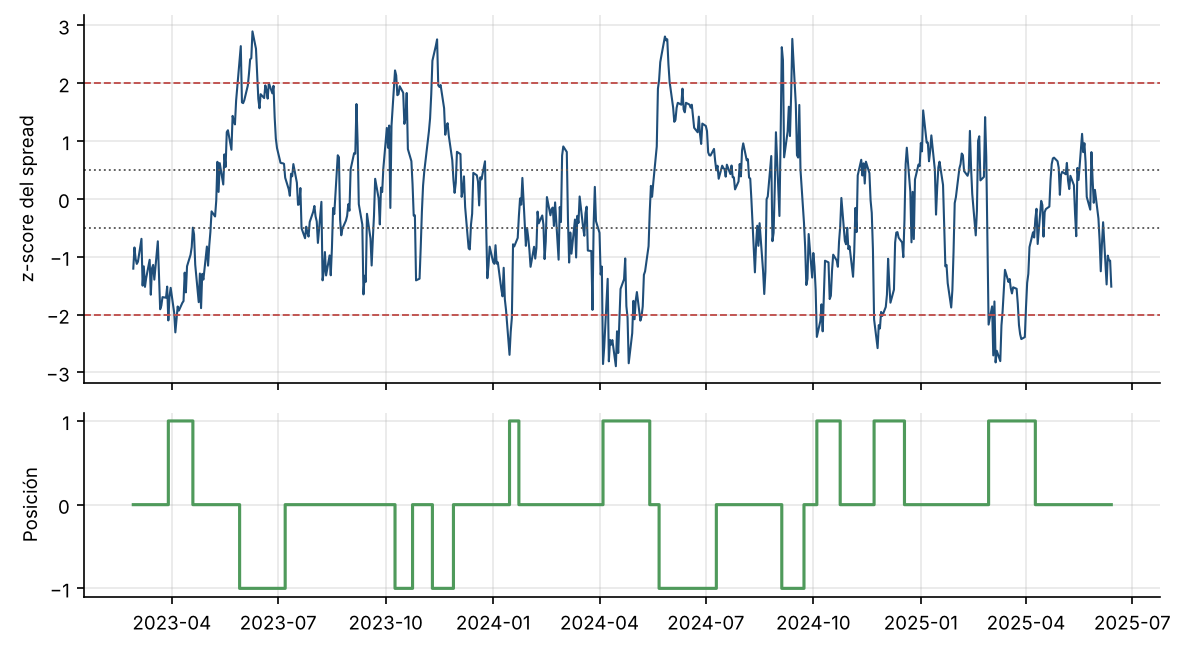
\includegraphics[width=0.9\textwidth]{f07_pares}
\caption{$z$-score de un spread cointegrado (fuera de la muestra de estimación de $\beta$) y la posición resultante.}
\end{figure}
\begin{aviso}
La cointegración se rompe (OPAs, cambios de negocio, crisis). Pon siempre un stop en $z$ (p.~ej. $|z|>4$)
y en tiempo (3--4 vidas medias).
\end{aviso}

\begin{ejercicios}
\begin{enumerate}
\item Calcula la beta de una acción con \py{equity.capm} sobre tus datos. ¿Cuántos contratos de futuro
  del índice cubren una cartera de 500\,000~\$ con beta 1,2 si el futuro tiene nocional 250\,000~\$?
\item Ejecuta \py{python scripts/backtest.py --estrategia pares} y relaciona la vida media con la duración de las operaciones.
\end{enumerate}
\end{ejercicios}
